%%%%%%%%%%%%%%%%%%%%%%%%%%%%%%%%%%%%%%%%%%%%%%%%%%%%%%%%%%%%%%%%%%%%%%%%%%%%%%%%
%2345678901234567890123456789012345678901234567890123456789012345678901234567890
%        1         2         3         4         5         6         7         8

\documentclass[letterpaper, 12 pt, conference]{ieeeconf}  % Comment this line out
                                                          % if you need a4paper
%\documentclass[a4paper, 10pt, conference]{ieeeconf}      % Use this line for a4
                                                          % paper

\IEEEoverridecommandlockouts                              % This command is only
                                                          % needed if you want to
                                                          % use the \thanks command
\overrideIEEEmargins
% See the \addtolength command later in the file to balance the column lengths
% on the last page of the document



% The following packages can be found on http:\\www.ctan.org
\usepackage{graphicx} % for pdf, bitmapped graphics files
\usepackage{bm}
\newcommand{\uvec}[1]{\boldsymbol{\hat{\textbf{#1}}}}
%\usepackage{epsfig} % for postscript graphics files
%\usepackage{mathptmx} % assumes new font selection scheme installed
%\usepackage{times} % assumes new font selection scheme installed
%\usepackage{amsmath} % assumes amsmath package installed
%\usepackage{amssymb}  % assumes amsmath package installed

\title{\LARGE \bf
Puzzle Encryption Algorithm : A Symmetric
variable size Block Cipher for data encryption
}
%\author{ \parbox{3 in}{\centering Gregory Alvarez, Charles Berenguer*
%         \thanks{*Use the $\backslash$thanks command to put information here}\\
%         Goswell Security Laboratory\\
%         {\tt\small gregory.alvarez@goswell.net}}
%         {\tt\small charles.berenguer@goswell.net}}
%        35 rue Lauriston, 75016 Paris, France \\
%}

\author{Utkarsh Bhandari$^{1}$ % <-this % stops a space
\thanks{}% <-this % stops a space
\thanks{$^{1}$ Utkarsh Bhandari, BT18CSE006, Department of Computer Science and Engineering,NIT Uttarakhand}%
\thanks{}%
}

\begin{document}

\maketitle
\section{Abstract}
The underlying structure of network security mainly consists of encryption algorithms. These algorithms are broadly divided into two categories symmetric encryption algorithm and asymmetric encryption algorithm both having their own pros and cons. In this algorithm the sender and the receiver receive the same key which is why it symmetric encryption approach . The objective of the paper is to delineate the security of the algorithm. The strength of the algorithm is tested by using various cryptanalytic attacks such as  Linear, Brute force, Differential, Differential-linear Crypt-analysis.
The scrupulous juxtaposition of the puzzle encryption with the Advanced Encryption Standard (AES) which is yet another method to encrypt data, is a vital ground for exegesis.  
The algorithm has some interesting properties: Variable block size, Key size is erratic and the algorithm is much faster than the average cryptography function. The algorithm is created while acknowledging the concepts of Confusion and Diffusion and the observable universe.
The cryptography is non-linear and is multi-operational on bits as well as bytes.

\section{Introduction}
Puzzle uses transposition rather than substitution. It is a variable block cipher algorithm and uses the following formula to rearrange the plaintext:
\\encryptedIndex=(plainIndex*(No. of key bytes)+other key bytes)mod(size of current block)\\
where encryptedIndex represents the final index and plainIndex represents the initial  index.
The idea behind this formula is like shuffling the lines of a program to a point that it does not make sense. This makes reversing the process convoluted and difficult to interpret, without the password. This is one-way encryption.\\ 

The algorithm involves the following steps: \\*
\begin{enumerate}
\item Key generation
\item Block size calculation
\item XOR with plaintext
\item Creation of MAP
\item Methods for encryption and decryption
\end{enumerate}
\begin{center}
    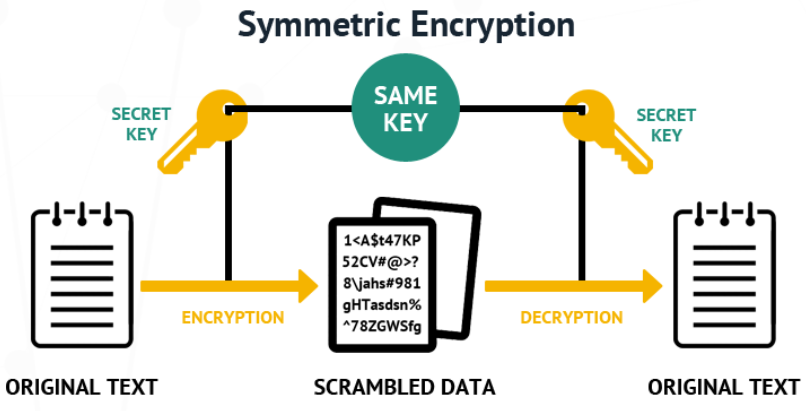
\includegraphics[width=.5\textwidth]{USELR1.PNG}
\end{center}



\section{Literature Survey}
The key generations utilized in Puzzle Encryption algorithm and different Symmetric Encryption algorithms are disparate. The [3] and [4] references, expounds the idea about how various symmetric encryption algorithms generate the key value and the time taken by them. Puzzle encryption algorithm beats most of the other algorithms with regards to security and speed, except Advanced Encryption Standard abbreviated as AES. Parts of the key are hashed and are then concatenated together. There has been no information regarding the use of rounds in the paper. For prevention of brute force attacks, we need to iterate on a reverse pass.\\
Since the aforementioned algorithm, AES is perfect and cannot be broken by any method in present date this method has used another approach similar to AES but not as good as AES, when it comes to functionality. The originality of this paper comes from a Promethean method of key generation and positioning of each plaintext character at wavering positions in the ciphertext.\\
\\
References [5] and [6] provides a thorough explanation of the comparison of asymmetric and symmetric algorithms. It asserts on how AES is faster, cheaper, more secure and has low power consumption as compared to Data Encryption Standard(DES) and Asymmetric Algorithms like Diffie Hellman and RIVEST-SHAMIR-ADLEMAN Algorithm. So, after a comparative study it can be proved that the puzzle encryption algorithm will also be advantageous when compared to these algorithms.
\\
Now, one may question the advantages of Puzzle over AES. Refrence [7] cites how with developing technology, security becomes a major concern while handling data. It gives germane details about how, having random block size and random key length can be advantageous. Puzzle providing these features can increase the scope for development of AES.

When the cipher-text is reordered 
The Security of the algorithm is the difficulty of repossession of the initial position of an element in the ciphertext. For example, without any changes to the plaintext(E.g. "MMMMM"), the output ciphertext will be same as the plaintext.
So in accordance to Shanon’s principle of Confusion and Diffusion the plaintext is XOR’ed with the first final key.
Further analysis of the paper will be done in the next section.


\section{Implementation}
\subsection{Key Generation}
The first step in implementation is key generation which involves hashing blocks of password and concatenating them together. After this chosen three letter group is hashed and added to the key. Since this three letter hash can be easily recovered by brute force, it becomes absolutely necessary to have an additional pass in reverse order. This algorithm requires two keys. One key is for XOR operation with plain-text and other one is to produce the mapping between final and initial position. Here the second key is generated in the same way as written above but with the reversed password.
\subsection{Block Size Calculation}
The Second Final Key is then used to calculate the block size by using each bit of the key which is not known to the attacker. The minimum block size allowed for a byte mapping (100 bytes) are 100 elements.
\subsection{Plaintext XOR}
The First final key is XOR'ed with the plaintext. This step is done for obscuring the plaintext with regards to Shannon's principle [2]: Confusion and Diffusion.
\subsection{Map Creation}
There are two methods of creating a map which links the initial and final positions: Unfolding of memory and iteration.


\section{Drawbacks}
The paper states that the encryption of data smaller than established limit is dangerous as it makes it easier to brute-force. If bits are used instead of bytes the encryption becomes more secure, but this engenders the problem of movement of a single bit around memory which in turn, slows the process by adding more processor operations. It states that encryption/decryption process needs up to twice or four times the block size in memory. 

\section{Cryptanalysis}
\subsection{Brute Force}
The algorithm cannot be deciphered by Brute force, except if the hacker knows some part of the plaintext. If a 5 word password is used with 512 bit hashing algorithm, it will create a 1024 bit key, which will create 10$^{308}$ combinations.
The key size not known, will eventually result in an increase in the number of combinations, exponentially. Even if 50 supercomputers are used to break a 256 bit key, with each calculating 10$^{18}$ combinations per second, will take 10$^{51}$ years to break.
\subsection{Linear Cryptanalysis} 
Since the algorithm has a non-linear characteristic: shifting of plaintext before XOR, unknown key size,increase in intial position of an element in the plaintext, it makes it impossible to break using linear cryptographic techniques.
\subsection{Differential Cryptanalysis} 
Many steps during the encryption process make it impossible to break using differential cryptanalysis: Shifting of plaintext before being XORed, not resetting the position of the first final key after every block, the non-linearity of the algorithm makes it impossible to recover an associated part of the key even if the initial and final position of an element is known, the relation will be only valid for the present block.
\subsection{Differential-Linear Cryptanalysis}
The non-linearity of the algorithm creates a condition in which an equation cannot be created to link the plaintext to the cipertext and the positioning of characters. Therefore such kind of attack is also not possible.
\newpage
\begin{thebibliography}{99}
	\bibitem{c6} 
	Alvarez, Gregory, and Charles Berenguer. "Puzzle Encryption Algorithm." arXiv preprint arXiv:1309.2103 (2013).
	\bibitem{c3} 
	http://en.wikipedia.org/wiki/Confusionanddiffusion
	\bibitem{c2}
	Agrawal, Monika, and Pradeep Mishra. "A comparative survey on symmetric key encryption techniques." International Journal on Computer Science and Engineering 4.5 (2012): 877.
	\bibitem{c6}
	Abd Elminaam, Diaa Salama, Hatem Mohamed Abdual-Kader, and Mohiy Mohamed Hadhoud. "Evaluating the performance of symmetric encryption algorithms." IJ Network Security 10.3 (2010): 216-222.
	\bibitem{c6}
	Bhanot, Rajdeep, and Rahul Hans. "A review and comparative analysis of various encryption algorithms." International Journal of Security and Its Applications 9.4 (2015): 289-306.
	\bibitem{c6}
	Bisht, Nivedita, and Sapna Singh. "A comparative study of some symmetric and asymmetric key cryptography algorithms." International Journal of Innovative Research in Science, Engineering and Technology 4.3 (2015): 1028-1031.
	\bibitem{c6}
	D'souza, Flevina Jonese, and Dakshata Panchal. "Advanced encryption standard (AES) security enhancement using hybrid approach." 2017 International Conference on Computing, Communication and Automation (ICCCA). IEEE, 2017.
	\bibitem{c6}B. Schneier, Applied cryptography, Wiley, 1996.
    \bibitem{c4}J.A. Buchmann, Introduction to Cryptography, Springer, New York,1999.
    \bibitem{c5}J. Hoffstein, J. Pipher, J.H. Silverman, An introduction to mathematical cryptography, Springer, New York, 2008.
    \bibitem{c6}A.J. Menezes, P.C.V. Oorschot, and S.A. Vanstone. Handbook Of Applied Cryptography. CRC Press, 1997.
	\bibitem{c6}B. Schneier, Applied cryptography, Wiley, 1996.
	
	
\end{thebibliography}
\end{document}
